\documentclass[a4paper,12pt]{article}
\usepackage{hyperref}
\usepackage{fullpage}
\usepackage{caption}
\usepackage{subcaption}
\usepackage{url}
\usepackage{graphicx}
\usepackage{hyperref}
\usepackage{listings}
\usepackage{color}
\usepackage{listings}
\usepackage{color}
\usepackage{amsmath}
\usepackage{amssymb}


\author{Paul Rubenstein\\ \texttt{pkr235@cam.ac.uk} \and Steve Smith \\ \texttt{sps41@cam.ac.uk} \and Argyris Zardilis \\ \texttt{az325@cam.ac.uk}}
\title{Systems Biology Assignment}

\begin{document}
\maketitle

\section*{Question 1}
\subsection*{A}
\[f(x) = \lambda \frac{K^n}{K^n + x^n}\]
\underline{Claim:} The log-log sensitivity of $f(x)$ is bounded (below) by $-n$.

\noindent \underline{Proof:} 
\begin{align*}
\frac{\partial \ln f}{\partial \ln x} & =  \frac{\partial f(x)}{\partial x}\frac{x}{f(x)} \\
& = \frac{\partial (\lambda \frac{K^n}{K^n + x^n})}{\partial x} \frac{x(K^n + x^n)}{\lambda K^n} \\
& = \frac{- \lambda K^n n x^{n-1}}{(K^n + x^n)^2} \frac{x(K^n + x^n)}{\lambda K^n} \\
& = \frac{-n x^n}{K^n + x^n}\\
& = -n \cdot \frac{1}{(K/x)^n+1}
\end{align*}

Now $K, x, n \geq 0$ and hence the denominator in the preceding line is larger than 1. Thus:

\begin{align*}
\frac{\partial \ln f}{\partial \ln x} & = -n \cdot \frac{1}{(K/x)^n+1} \geq -n
\end{align*}

And thus the claim is true. $\square$

For an example plot of a Hill-type repression function, see Figures \ref{hill} and \ref{log-log}. Note that the log-log sensitivity tends to $-1$ as $x\longrightarrow \infty$

\begin{figure}
\centering
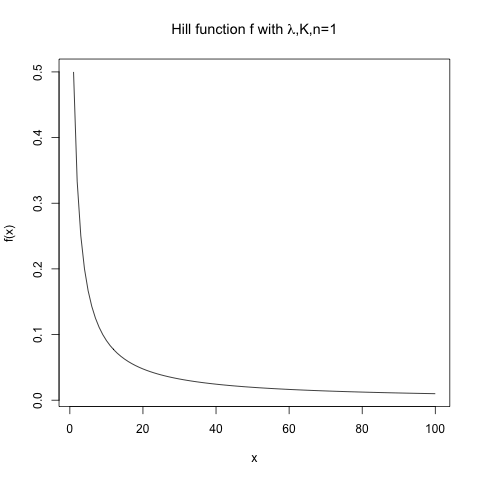
\includegraphics[width=5in]{images/hill.png}
\caption{A plot of the Hill function $f(x) = \lambda \frac{K^n}{K^n+x^n}$}
\label{hill}
\end{figure}

\begin{figure}
\centering
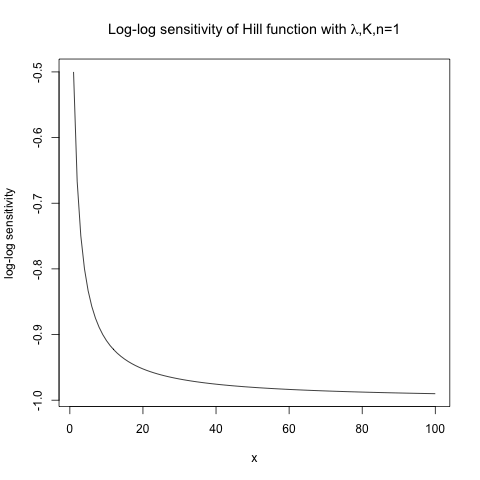
\includegraphics[width=5in]{images/log-log.png}
\caption{Log-log sensitivity of the Hill function $f(x) = \lambda \frac{K^n}{K^n+x^n}$. Note that the curve tends to $-1$ as $x\longrightarrow \infty$}
\label{log-log}
\end{figure}

\subsection*{B}

\underline{Claim:} \[f(x) = a x+b \Rightarrow \left \langle \frac{\Delta f / \langle f \rangle}{\Delta x / \langle x \rangle}  \frac{{\Delta x}^2}{\langle \Delta x^2 \rangle} \right \rangle = \frac{\partial \ln f}{\partial \ln x} \bigg|_{x=\langle x \rangle} \]

\noindent \underline{Proof:}

\[ \frac{\partial \ln f}{\partial \ln x} \bigg|_{x=\langle x \rangle} = \frac{\partial f}{\partial x} \frac{x}{f} \bigg|_{x=\langle x \rangle} = \frac{a\langle x \rangle}{a \langle x \rangle + b}\]

and

\[ \Delta f = f - \langle f \rangle = (ax+b) - (a \langle x \rangle - b) = a \Delta x\]

Thus:

\begin{align*}
\left \langle \frac{\Delta f / \langle f \rangle}{\Delta x / \langle x \rangle} \frac{{\Delta x}^2}{\langle \Delta x^2 \rangle} \right \rangle & = \left \langle \frac{a \Delta x /( a \langle x \rangle - b)}{\Delta x / \langle x \rangle} \frac{\Delta x ^2}{\langle \Delta x ^2 \rangle} \right \rangle \\
&= \left \langle \frac{a \langle x \rangle}{a \langle x \rangle - b} \frac{\Delta x ^2}{\langle \Delta x ^2 \rangle} \right \rangle \\
&= \frac{a \langle x \rangle}{a \langle x \rangle - b} \frac{\langle \Delta x ^2 \rangle}{\langle \Delta x ^2 \rangle} = \frac{a \langle x \rangle}{a \langle x \rangle - b} = \frac{\partial \ln f}{\partial \ln x} \bigg|_{x=\langle x \rangle}
\end{align*}

Since $a, \langle x \rangle$ and $\langle \Delta x^2\rangle$ are constants. Thus the claim is true.  $\square$

\subsection*{C}

The difference between the two corrective measures - the overall corrective tendency and the log-log sensitivity - is that the former is `the true behaviour of the system' whereas the latter is used as an approximation to the former as it is easier to calculate and use in analysis. Part B above shows that in the case that $f$ is a linear function of $x$, the two quantities are equal. If $f$ is well-behaved near the stationary value for $x$ and the fluctuations are small we can approximate $f$ by a linear function of $x$ by Taylor's theorem. Thus we can use $\frac{\partial \ln f}{\partial \ln x}$ as a valid approximation to the true corrective function in this case.


\section*{Question 2}

\subsection*{A}
The simulation (code attached) results using a variety of parameter values for each variable are displayed graphically in figure~\ref{fig:vars}. They show that, for fixed $C$, the fluctuations are larger for small $\lambda$ and large $\beta$ and smaller for large $\lambda$ and small $\beta$. 

When $C$ and $\beta$ are large compared to $\lambda$ there appears to be little correlation between the values of $C$ and $\beta$ and the observed fluctuations. When $C$ and $\beta$ are small compared to $\lambda$ we see that smaller $C$ and $\beta$ lead to smaller fluctuations and we see that larger $C$ and $\beta$ lead to larger fluctuations.

When $C$ and $\lambda$ are small compared to $\beta$ we see that smaller values of $\lambda$ lead to larger fluctuations and that the value of $C$ is correlated positively with the magnitude of the fluctuations for fixed $\lambda$ but that its effect on the fluctuations is smaller than that of $\lambda$.

When $\lambda$ is increased or $\beta$ or $C$ are decreased it is clear that $\langle x \rangle$ should increase, since changing these parameters in this way affects the overall production/destruction rate predictably. It is less clear what effect changing these parameters will have on $\sigma^2_x$, and since the relative deviations depend on both of these quantities numerical simulation or mathematical arguments are needed to understand the effect of changing parameters. For example, for fixed $\beta$ and $C$ it is not intuitively clear what effect increasing $\lambda$ would have on $\sigma^2_x$ - however from the figures we can infer that either $\sigma^2_x$ is decreasing or it is increasing at a slower rate that $\langle x \rangle$.

\begin{figure}[!ht]
        \centering
        \begin{subfigure}[b]{0.49\textwidth}
                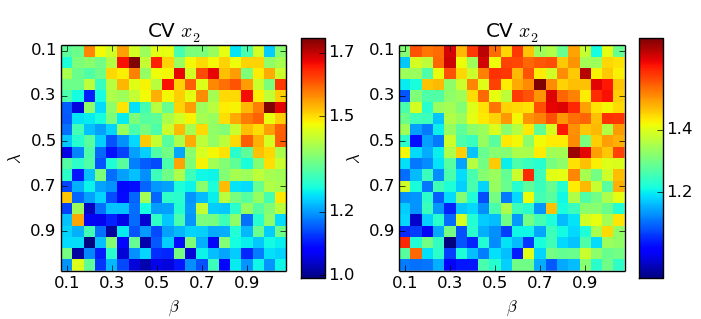
\includegraphics[width=\textwidth]{images/vars1}
                \caption{$\lambda, \beta < C=1.5$}
                \label{fig:vars1}
        \end{subfigure}%
        \hfill
        \begin{subfigure}[b]{0.49\textwidth}
                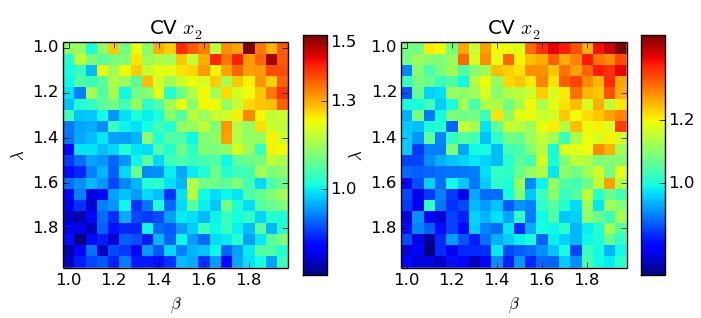
\includegraphics[width=\textwidth]{images/vars2}
                \caption{$\lambda, \beta > C=0.5$}
                \label{fig:vars2}
        \end{subfigure}
          \newline
        \begin{subfigure}[b]{0.496\textwidth}
        \centering
                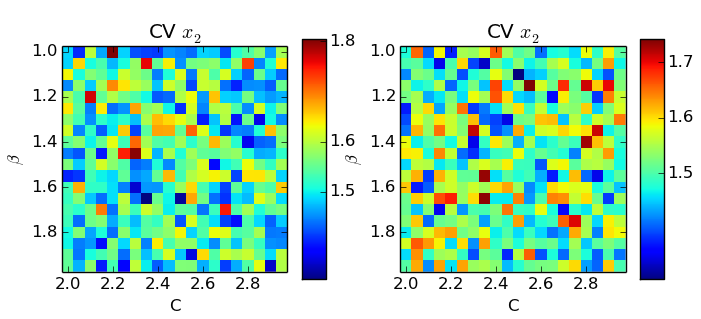
\includegraphics[width=\textwidth]{images/vars3}
                \caption{$C, \beta > \lambda=0.5$}
                \label{fig:vars3}
        \end{subfigure}
        \begin{subfigure}[b]{0.496\textwidth}
                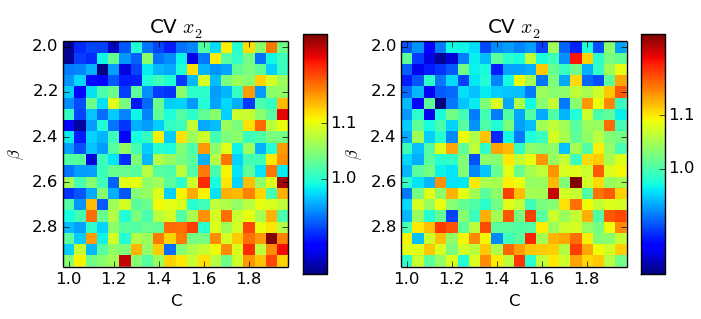
\includegraphics[width=\textwidth]{images/vars4}
                \caption{$C, \beta < \lambda=3.0$}
                \label{fig:vars4}
        \end{subfigure}
          \newline
        \begin{subfigure}[b]{0.496\textwidth}
                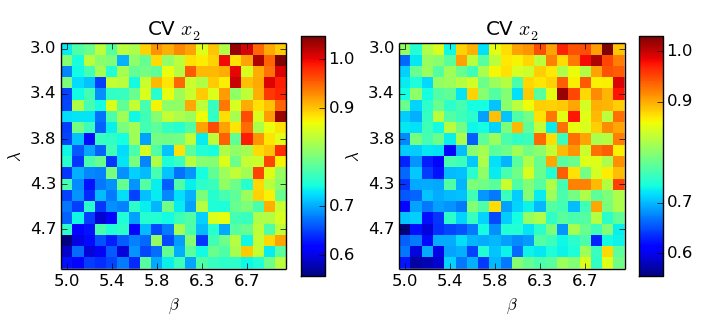
\includegraphics[width=\textwidth]{images/vars5}
                \caption{$\lambda, \beta > C=1.0$}
                \label{fig:vars5}
        \end{subfigure}
        \begin{subfigure}[b]{0.496\textwidth}
                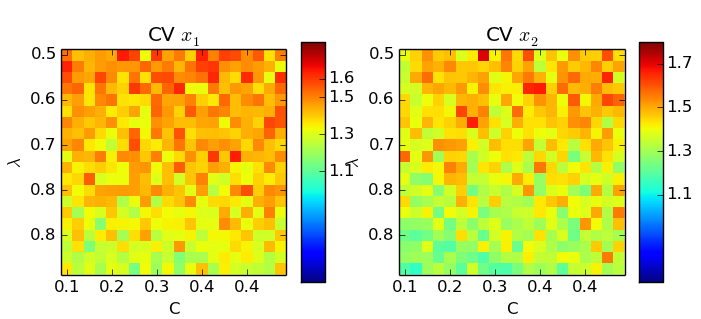
\includegraphics[width=\textwidth]{images/vars6}
                \caption{$C, \lambda < \beta=5.0$}
                \label{fig:vars6}
        \end{subfigure}
        
        \caption{CVs of the two species, $x_1$ and $x_2$, for different parameter regimes. For each parameter regime one of the 3 parameters was kept constant with the other 2 varying over a $20 \times 20$ grid of values.}\label{fig:vars}
\end{figure}

\subsection*{B}
Figure~\ref{fig:dev_hists} demonstrates the symmetry of the system in the numerical simulations. Both variance and expectation differences are distributed about 0 with a small spread. Since the simulations are stochastic it is not surprising that there are non-zero differences in either the variance or expectations, however we do require that the expectations of these differences are 0  - something that we do see. Similarly figure~\ref{fig:?} confirms that the requirement that flux balances are maintained at stationarity is met, with the relative deviations being minimal and centered symmetrically around 0.


\begin{figure}[!ht]
        \centering
        \begin{subfigure}[!ht]{0.7\textwidth}
                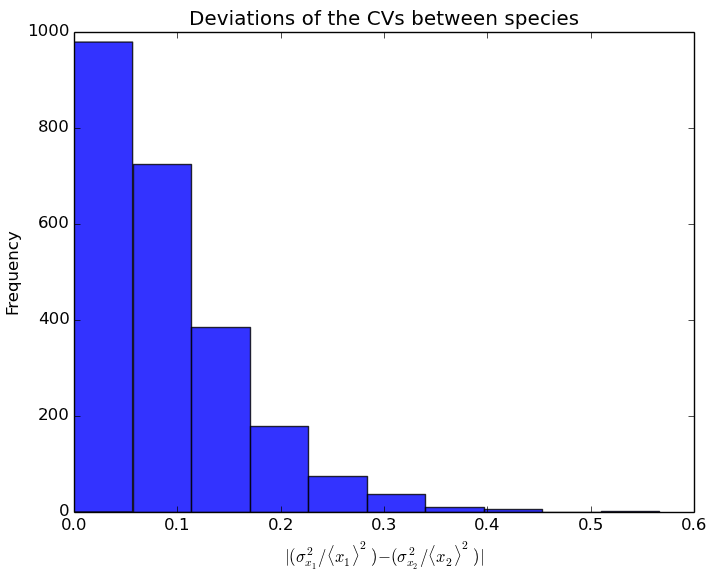
\includegraphics[width=\textwidth]{images/vars_devs}
                \caption{}
                \label{fig:devs_vars}
        \end{subfigure}%
        
        \begin{subfigure}[b]{0.7\textwidth}
                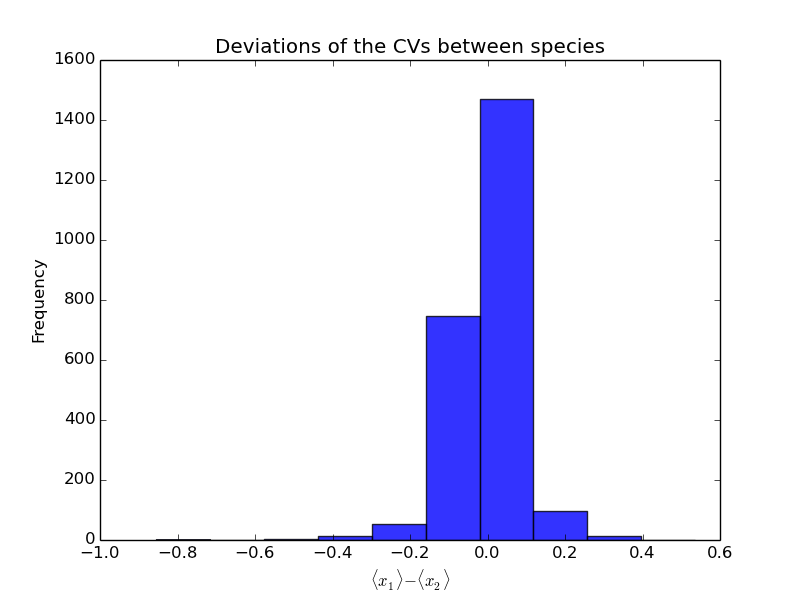
\includegraphics[width=\textwidth]{images/avgs_devs}
                \caption{}
                \label{fig:devs_avgs}
        \end{subfigure}
        
\caption{Relative deviations of the CVs (a) and averages (b) between the two subunits over a number of simulations.}
\label{fig:dev_hists}
\end{figure}

\subsection*{C}
Figure~\ref{fig:approx_exact_var} compared the approximate and exact variances directly, whilst figure~\ref{fig:approx_var_dev} shows the frequencies of deviation between the two. Together they show that the approximation is consistantly higher than the exact variance, with the over-estimation becoming larger as the exact variance increases. 

There may not be a causal link between larger exact variances and worse over-estimation; it may have arisen due to the choice of parameters used. The difference between the exact and inexact variances can be traced to the approximation used to calculate the efficiency $E$ in which we assume that $\langle x_1 x_2 \rangle = \langle x_1 \rangle \langle x_2 \rangle$. This is a true equality in the case that $x_1$ and $x_2$ are independent and is a worse approximation the greater the correlation between the two. When we examined the points in figure~\ref{fig:approx_exact_var} we found that those with approximate variances greater than $3$ all came from simulations with parameters in which $\beta$ was very small and $C$ was very large. In this case $x_1$ and $x_2$ are strongly correlated (because a decrease in $x_1$ probably comes about from a reaction that also decreases $x_2$) and so the approximation is less valid. This may explain why the variances for these points were overestimated so much more than the rest.

It is worth pointing out that despite inaccuracies for certain choices of parameters, there are many cases in which the approximations are accurate enough to be useful.

\begin{figure}[!ht]
        \centering
        \begin{subfigure}[!ht]{0.7\textwidth}
                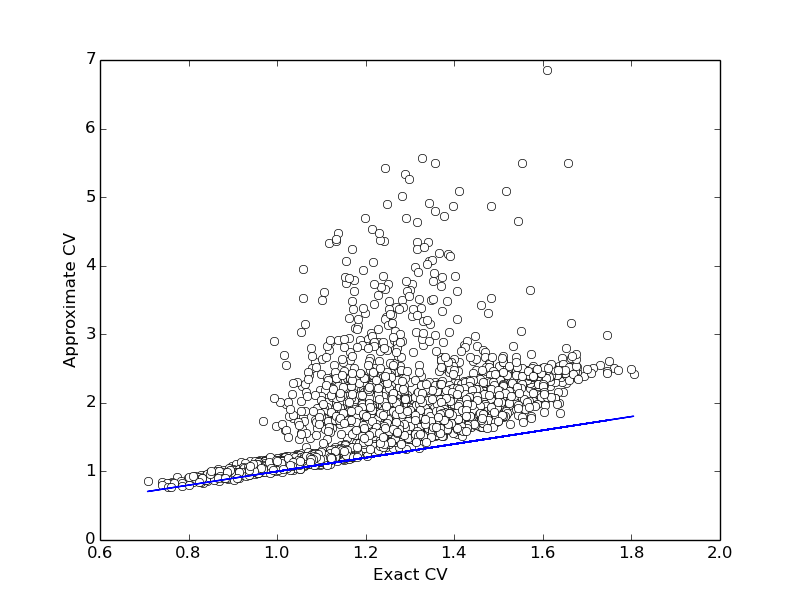
\includegraphics[width=\textwidth]{images/approx_exact_var}
                \caption{}
                \label{fig:approx_exact_var}
        \end{subfigure}%
        
        \begin{subfigure}[b]{0.7\textwidth}
                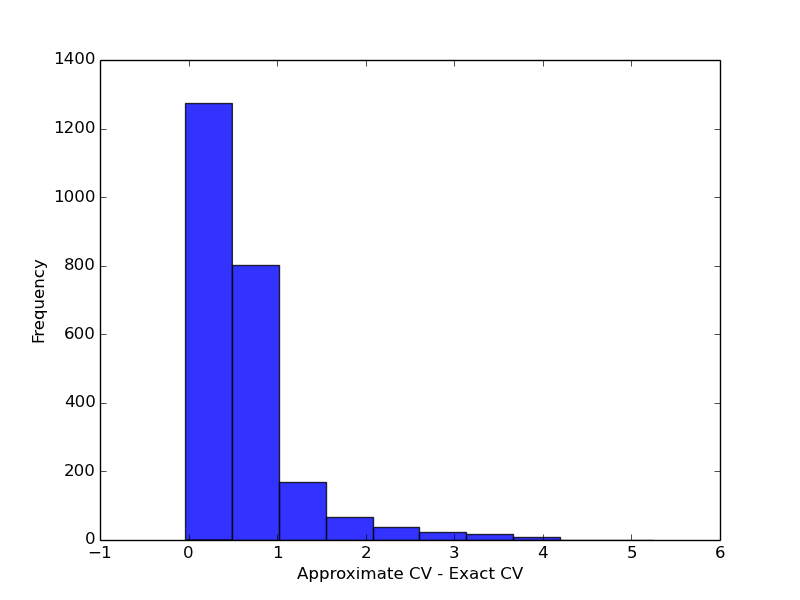
\includegraphics[width=\textwidth]{images/approx_var_dev}
                \caption{}
                \label{fig:approx_var_dev}
        \end{subfigure}
        
\caption{(a) Plot of approximate against exact variances (line is $y=x$) and (b) histograms of the deviations between the two. Exact and approximate variances were calculated for 2400 simulation each with different parameter sets.}
\label{fig:dev_hists}
\end{figure}









\end{document}